\begin{activity} \label{A:11.8.2} A picture of a cylindrical box, 
$B = \{(r,\theta,z) : r_1 \leq r \leq r_2, \theta_1 \leq \theta \leq \theta_2, z_1 \leq z \leq z_2\},$
is shown in Figure \ref{F:11.8.Cylindrical_Vol_Element}. Let $\Delta r = r_2-r_1$, $\Delta \theta = \theta_2 - \theta_1$, and $\Delta z = z_2-z_1$. We want to determine the volume $\Delta V$ of $B$ in terms of $\Delta r$, $\Delta \theta$, $\Delta z$, $r$, $\theta$, and $z$.
\begin{figure}[ht]
\begin{center}
%\resizebox{!}{2.5in}{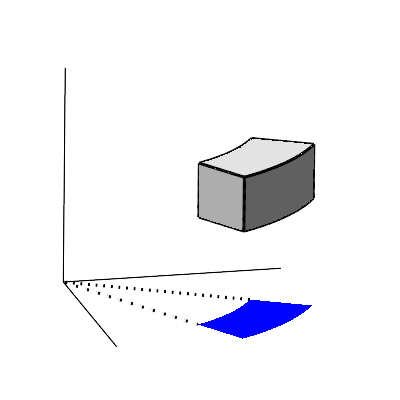
\includegraphics[trim=1.0cm 1.5cm 1.0cm 1.5cm, clip]{11_8_Cylindrical_volume_element}}
  
\includegraphics{figures/fig_11_8_cylindrical_box.eps}
\end{center}
\caption{A cylindrical box.}
\label{F:11.8.Cylindrical_Vol_Element}
\end{figure}
%crop graphics in animate trim=<left> <bottom> <right> <top>, clip with includegraphics

    \ba
    \item Appropriately label $\Delta r$, $\Delta \theta$, and $\Delta z$ in Figure \ref{F:11.8.Cylindrical_Vol_Element}.



    \item Let $\Delta A$ be the area of the projection of the box, $B$, onto the $xy$-plane, which is shaded blue in Figure \ref{F:11.8.Cylindrical_Vol_Element}.  Recall that we previously determined the area $\Delta A$ in polar coordinates in terms of $r$, $\Delta r$, and $\Delta \theta$. In light of the fact that we know $\Delta A$ and that $z$ is the standard $z$ coordinate from Cartesian coordinates, what is the volume $\Delta V$ in cylindrical coordinates?



    \ea


\end{activity}
\begin{smallhint}

\end{smallhint}
\begin{bighint}

\end{bighint}
\begin{activitySolution}
    \ba
    \item The labels are shown below. 
\begin{center}
\resizebox{!}{2.5in}{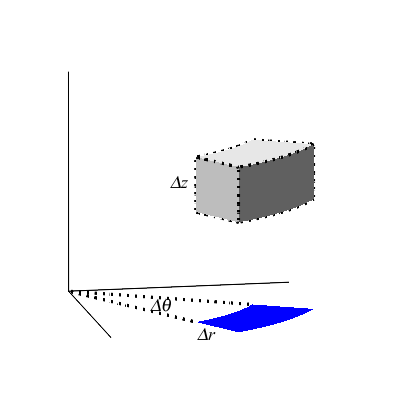
\includegraphics[trim=1.0cm 1.5cm 1.0cm 1.5cm, clip]{11_8_cbox_labels}}
\end{center}

    \item Recall that $\Delta A$ was $\frac{1}{2}(r_{i+1}+r_i) \Delta r \ \Delta \theta$. Since $z$ is just the standard height, we have 
\[\Delta V = \Delta A \ \Delta z = \frac{1}{2}(r_{i+1}+r_i) \Delta r \ \Delta \theta \Delta z.\]

    \ea
\end{activitySolution}
\aftera

